
\chapter{\label{cha:pgraph}PGraph and PNS}

 
In a process system , raw materials are consumed through various transformation to yield desired products . 
This is usually accompanied bu the generation of wastes .Vassels in which these transformations are carried out are termed operating units of the process , a given set of operating units with the plausible interconnections can be described bu a network The desired products can often be manufactured using some sub networks of this network , thus a given network may give rise to a variety of processes producing the desired products , and each of such process corresponds to sub network which can be considered  to be its structure
\section{ PGraph }


The so called P graph (Process graph), which is a directed bigraph, has been used for modelling network structures for some time.
The vertices of the graph denote the operating units (O   operating units) and the materials (M   materials).
The edges of the graph represent the material-flow between the materials and the operating units.
\subsection{ General Definition of P-Graph }

The Pgraph is a bigraph, meaning that its vertices are in disjunctive sets and there are no edges between vertices in the same set.
In case of P graphs the assignment of operating units and materials are strictly determined by the tasks given, i.e. an edge can point to an M material type vertex from an O operating unit type vertex, only if M is element of the output set of O, that is O produces M material namely, M $\in$ output O . 


An edge can point from an M material type vertex to an O operating unit type vertex, only if M is element of the input set of O, that is O processes M material, namely M  $\in$ input O. .
Thus, the P-graph can be presented by the pairs of operating unit and the assigned material vertices set like the (M,O) P-graph.
The material type vertices can be put into several subsets. 
There are various subsets like the raw-material type one, which contains the input elements of the whole process, the product-material type subset, which gathers the results of the entire process, the intermediate-material type one, the elements of which emerge or are used between the processing phases, and finally the by-product-material  type set, which contains the non desired results of the process. The applied operating unit and material element notations in the P-graph notation are presented in \ref{fig:example for P-graph}.

As an example let us consider a process network with 7 operating units, in which the operating units are 1,2....7 and the materials are A,B, .... L. A,B,C and D are the materials available for the production of L The possible structure is given in  .

\begin{figure}[th]
	\centering
		\includegraphics{chapiter2/img/notationP}
	\caption{\label{fig:notation in pgraph}notation in pgraph}
\end{figure}


\begin{figure}[th]
	\centering
		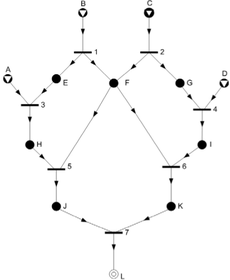
\includegraphics{chapiter2/img/examplePgraph}
	\caption{\label{fig:example for P-graph}example for P-graph }
\end{figure}

\section{ Process Network Synthesis }

In the Process Network Synthesis (PNS for short) problem a set of materials is given and also operating units 
which are transforming some subset of materials into some other subset.
The subsets assigned to the operating unit are called its  input and output materials. 
In the problem two subsets of the materials are distinguished, 
one is the set of the raw materials and the other is the set of the desired products.
Our goal is to find a minimal cost network of the operating units which can produce all desired products starting from the raw material. These systems can be modeled in the P-graph framework which is based on bipartite graphs.


In these P-graphs we have two sets of vertices, one of them contains the possible materials,
the other the operating units. The edges lead to an operating unit from its input materials 
and from an operating unit to its output materials. 


Then the subgraphs satisfying some properties describe the feasible processes
which produce the desired products from the raw materials.
Thus our goal is to find the least expensive such subgraph. 
In the structural model the amounts of the material flows are not taken into account thus the cost of an operating unit is a constant, and the cost of a subgraph is the sum of the costs of the operating units contained in it. 
\subsection{ Basic Notation }

The structural PNS problem can be modeled in the PGraph framework.
In the PGraph (Process Graph) we have the set of the materials denoted by M,
which contain two special subsets, the set of raw materials and the set of desired products denoted by R and P respectively

The problem also contains a set of possible operating units which can transform some sets of materials. 

The set of operating units is denoted by O. An operating unit u is given by two sets, 
in(u) denotes the set of the input materials out(u) denotes the set of output materials of the operating unit

This means that the operating unit can work in a solution structure if all of its input materials are produced and in this case it 
produces all of its output materials. 

The PGraph  of the problem is defined by the sets M and O. It is a directed bipartite graph where the set of vertices is M $\cup$ O, and have the following two sets of edges:
\begin{enumerate}
\item Edges which connect the input materials to their operating unit
\item Edges which connect the operating units to their output materials
\end{enumerate}

Then some of the subgraphs of this P-graph describe the feasible solutions which produce the required materials from the raw materials.  
where m and o are the subsets of M and O, represent a feasible solution if and only if the following properties called axioms are valid: 
\begin{enumerate}

\item m contain all element of P    
\item a material from m is a raw material if and only if no edge goes into it in the P-graph (m, o)  
\item For each operating unit u from o there exists a path in the P-graph (m,o) which goes into a desired product from u  
\item m is the union of the input and output material sets of the operating units contained 
in set o  
 
\end{enumerate}

\subsection{Mathematical definition }

There is a finite set of material M (which contains the sets of P products and R raw-materials) 
and the finite set of O operating units. 
Consequently, the set of P end-products and the set of R raw-materials must be subsets of M 
and the set of M materials and the set of O operating units are disjunctive.
The basic relations between M,P,R and O are as follows : 

\begin{equation}
P\subseteq M,R\subseteq M,M\cup O=\emptyset\label{eq:1}
\end{equation}

As physical processes are defined, each operation unit produces output materials from
input materials. Therefore two disjunctive sets can be assigned to each operating unit, i.e. the set of input and the set of output materials. 

Let an arbitrary operating unit ( $\alpha$ , $\beta$), then $\alpha$ is the set of input materials which are processed by the 
($\alpha$ , $\beta$ ) unit and $\beta$is the set of output materials, which are produced by the given unit .


Considering the process-network the output materials of each operating unit are the inputs of different operating units. In general, it can be proved that 

\begin{equation}
O\subseteq \rho(M) \times  \rho(M)\label{eq:second}
\end{equation}

where O is the set of operating units, M is the set of materials and $\rho(M)$ is the power set, 
that is the set of subsets of M, and $\rho(M) \times  \rho(M)$ represents the set of $\rho(M)$ and $\rho(M)$ pairs

Supposing that there is a finite set m, which is a subset of M, i.e. it is true that m $\subseteq$ M 
and there is an o finite set, which is a subset of O, i.e. 
it is true that o $\subseteq$ O and supposing that there is such a material
which is an input for one or more operating units, and there is such material 
which is the output of one or more operating units, then :

\begin{equation}
o\subseteq \rho(m) \times  \rho(m)\label{eq:second}
\end{equation}


The PNS is defined as a bigraph, where the set of V vertices is made of the elements of the union of m and o that is

\begin{equation}
V = m \cup o\label{eq:nex}
\end{equation}
 
 

\subsection{ Algorithms MSG, SSG, and ABB }
PNS representation of a process network and the set of  axioms for solution structures, i.e.,
combinatorial feasible networks, render it possible to fashion the three mathematically rigorous algorithms:
MSG, SSG, and ABB. 

The algorithm MSG (Maximal-Structure Generation) generates the maximal structure (super-structure)
of a process synthesis network.
Also, 

the algorithm SSG (Solution-Structure Generation) generates the set of feasible process structures from the maximal structure,

which leads to the algorithm ABB (Accelerated Branch and Bound) for computing the n-best optimal solution structure
\subsubsection{Maximal-Structure Generation}
The maximal structure of the synthesis problem (P, R, O) contains all the combinatorially possible structures, which make the production of defined products possible from given raw-materials. Therefore, it certainly contains the optimal structure as well.

The first phase is the input phase, in which the synthesis problem is defined (P, R, O) such a way, that the set of M all the plausible materials, the set of P end-products 

The second phase is the elaboration of the input structure of the network, which is carried out by the linking of all the similar (same type) material type vertices.

The third phase is the elimination phase, where those materials and operating units are eliminated, which, taking the  axioms into account, are not and cannot be linked to the maximal structure for sure

During the fourth phase the vertices are linked again from level to level, starting from the highest, the end-product level.

The maximal structure generated this way contains all the combinatorially possible structures and all of its elements fulfil the  axioms.
\subsubsection{Maximal-Structure Generation}
The maximal structure generated by the MSG algorithm contains all such combinatorically possible network structures that are able to produce the end-product from the given raw-materials.

Consequently, it contains the optimal network as well. In most cases the optimalisation means to find the most cost effective solution.

The application of the SSG (Solution Structure Generation) algorithm enables the production of all the solution structures. The SSG is a new mathematical tool  which has been developed by Friedler et al.

\subsubsection{Accelerated Branch and Bound}

The branch-and-bound method has been widely used The method is reiterated here to facilitate formalization of the
accelerated branch-and-bound algorithm of PNS.
to Identify the optimal process from the maximal structure 


\subsection{ Comparaison PNS and PetriNet : }
\begin {table}[H] 
\begin{tabular}{cc}

\hline 
\textbf{Petri Net}  & \textbf{Process Network Synthesis}\tabularnewline
\hline 
Source Place  & Raw Material\tabularnewline
Normal Place  & Intermediate Material\tabularnewline
Sink Place  & Final Product\tabularnewline
Token in Place  & Requirement Flow \tabularnewline
Transition  & Operating Unit \tabularnewline
Weight of in or out edges of the  transition & producing rate of the operating unit\tabularnewline
\hline 
Modeling Parallel System  & Basically use for Chemical Reaction \tabularnewline
\hline 

\end{tabular}
\caption {Petri Net and PNS}
 
\end {table}

\section{Conclusion}
in this chapter , i presente the definition of second framework i use
PGraph and define the Process Network synthesis .
with some Algorithme applicable on PNS
to find the optimum structure